\section{Improper Integral}
	\subsection{Normal Infinite Integral}
	Formula:
	\begin{multicols}{2}
	\noindent
	\begin{equation}
	\int^{\infty}_cf(x)=\lim_{t\rightarrow-\infty}\int^t_cf(x)
	\end{equation}
	\begin{equation}
	\int_{-\infty}^cf(x)=\lim_{t\rightarrow-\infty}\int_t^cf(x)
	\end{equation}
	\end{multicols}
	\noindent c can be any constant.
	
	\begin{simple}{}{}
	Find:
	\begin{align*}
	\int^\infty_1\frac{1}{x^2}&=\lim_{t\rightarrow\infty}\int^t_1\frac{1}{x^2}\ dx\\
	&=\lim_{t\rightarrow\infty}\frac{1}{x^2}\Big|^t_1\\
	&=\lim_{t\rightarrow\infty}\left(\frac{1}{t^2}+\frac{1}{1}\right)\\
	&=\frac{1}{\infty}+\frac{1}{1}\\
	&=0+1\\
	&=1
	\end{align*}
	\end{simple}
	
	\subsection{Double Infinite Integral}
	Formula:
	\begin{equation}
		\int^\infty_{-\infty} f(x)=\lim_{t\rightarrow\infty}			\int^t_cf(x)+\lim_{t\rightarrow-\infty}\int^c_tf(x)
	\end{equation}
	\noindent c can be any constant.
	
	\subsection{Discontinuity}
	Given f(x) is continuous at all points between a and b except  at x=c\\
	\begin{equation}
	\int^b_a f(x)\ dx=\lim_{t\rightarrow c^+}\int^b_t f(x)+\lim_{t\rightarrow c^-}\int^t_a f(x)\ dx
	\end{equation}
	
	\subsection{Comparison Test}
	\begin{theorem}{}{}
	If $f_1{(x)}$ is always bigger than $f_2(x)$, then if $f_2(x)$ diverges, $f_1(x)$ must diverge. \\
	If $f_2{(x)}$ is always smaller than $f_1(x)$, then if $f_1(x)$ converge, $f_2(x)$ must converge.
	\end{theorem}
	
	\begin{simple}{}{}
	In figure 1 blue line represents $\displaystyle\frac{1}{\sqrt{x}}$ and red line represents $\displaystyle\frac{1}{x}$. Since $\displaystyle\frac{1}{x}$ diverges\footnotemark[3] $\displaystyle\frac{1}{\sqrt{x}}$ has to diverge.
	\begin{multicols}{2}
	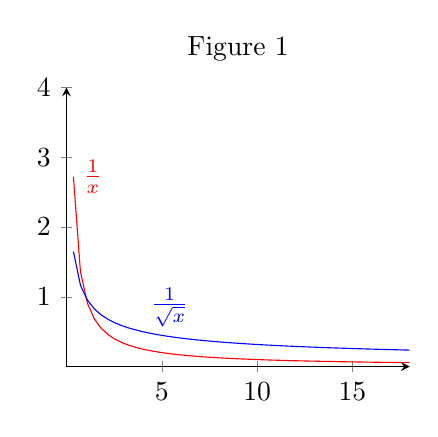
\begin{tikzpicture}
	\begin{axis}[width=0.49\textwidth, axis lines=middle, xmax=18, xmin=0, ymin=0, ymax=4, title=Figure 1]
	\addplot[color=red, domain=0:18, samples=50]{1/x}node[right, pos=0]{$\frac{1}{x}$};
	\addplot[color=blue, domain=0:18, samples=50]{1/sqrt(x)}node[pos=0.3, anchor=south]{$\frac{1}{\sqrt{x}}$};
	\end{axis}
	\end{tikzpicture}
	
	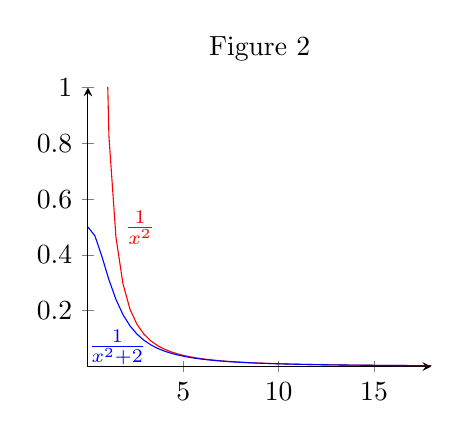
\begin{tikzpicture}
	\begin{axis}[width=0.49\textwidth, axis lines=middle, xmax=18, xmin=0, ymin=0, ymax=1, title=Figure 2]
	\addplot[color=red, domain=0:18, samples=50]{1/(x^2)}node[pos=0.3, anchor=west]{$\frac{1}{x^2}$};
	\addplot[color=blue, domain=0:18, samples=50]{1/(x^2+2)}node[pos=0.2, anchor=east]{$\frac{1}{x^2+2}$};
	\end{axis}
	\end{tikzpicture}
	\end{multicols}
	
	While in figure 2 blue line represents $\displaystyle\frac{1}{x^2+2}$ and red line represents $\displaystyle\frac{1}{x^2}$. Since $\displaystyle\frac{1}{x^2}$ converges\footnotemark[1] $\displaystyle\frac{1}{x^2+2}$ has to converge.
	\end{simple}
	
	\footnotetext[1]{Because of p-series}